\documentclass[aps,pra,reprint,superscriptaddress,longbibliography,nofootinbib]{revtex4-2}

\usepackage{amsmath,amssymb,mathtools}
\usepackage{bm}
\usepackage{graphicx}
\usepackage{microtype}
\usepackage[colorlinks=true,allcolors=blue]{hyperref}

\newcommand{\tr}{\operatorname{tr}}
\newcommand{\cD}{\mathcal D}
\newcommand{\cH}{\mathcal H}

\begin{document}

\title{Critical Sibuya quantum resetting converges on every fixed finite unitary register}

\author{Xiaojian Zeng}
\email{xiaojianzeng@foxmail.com}
\affiliation{PBC School of Finance, Tsinghua University, Beijing 100190, China}

\date{September 12, 2026}

\begin{abstract}
We consider exact discrete-time unitary dynamics interrupted by unconditional
resets to a fixed pure state.  The reset hazard after $n$ consecutive unitary
steps is $r_n=\gamma/(n+1)$, with $0<\gamma<1$, so the inter-reset time has
infinite mean.  For every fixed finite-dimensional unitary, we prove that the
ensemble density operator converges in Schatten trace norm to the pinching of
the reset state onto the distinct eigenspaces of the unitary.  The proof gives
a nonasymptotic bound controlled by the occupied eigenphase chord gaps and by
the two endpoint masses of the critical Sibuya age distribution.  At a fixed
nonzero gap, each coherence has two algebraic contributions, proportional to
$t^{\gamma-1}$ and $z^t t^{-\gamma}$, from distinct unit-circle singularities.
For $\gamma=1/2$ and eigenphase ratio $z=-1$, every odd-time coherence vanishes
exactly, whereas the even-time coefficient is a central binomial coefficient.
The estimates concern the ordinary time sequence, not only an Abel limit or
an adjacent-time diagnostic, and are intentionally nonuniform when an occupied
eigenphase gap closes.
\end{abstract}

\maketitle

\section{Introduction}

Stochastic resetting replaces part of a system's history by repeated returns
to a prescribed state.  In a quantum register, unitary gates between reset
events make the resulting ensemble a renewal mixture of coherent orbits.
For a constant reset probability, the geometric age distribution gives a
stationary state directly.  Age-dependent reset probabilities are subtler:
the age process is non-Markovian after the quantum state alone is retained,
and an infinite-mean renewal law can keep appreciable weight at both ends of
the available age interval.

Wald \emph{et al.} formulated a discrete-time quantum reset model and studied
both constant and age-dependent hazards~\cite{Wald2025}.  For the power-law
hazard $r_n=\gamma/(n+1)^\alpha$, their survival analysis and two-qubit
adjacent-time numerics indicate relaxation at the critical exponent
$\alpha=1$.  A vanishing adjacent difference does not, by itself, establish
convergence of the ordinary state sequence.  Independently, Michelitsch
\emph{et al.} derived the Sibuya backward-age distribution and its double
generating function for discrete resetting on networks~\cite{Michelitsch2025}.
Their displayed relaxation formula treats transform arguments strictly inside
the unit disk; nontrivial unitary eigenphases lie on its boundary.  A related
continuous-time quantum renewal model reaches a diagonal ensemble under a
final-value assumption~\cite{Sevilla2023}, but it does not provide the
discrete critical ordinary-time bound considered here.

This paper resolves the critical finite-register question.  The key elementary
observation is that, at fixed clock time, the exact Sibuya age mass is
U-shaped.  Its total variation is therefore bounded by its two endpoint
masses.  Discrete summation by parts turns that fact into a Fourier bound at
every nontrivial unit-modulus argument.  A spectral-block decomposition then
lifts the scalar estimate to Schatten trace norm.  We also retain both
boundary singularities of the generating function, which identifies the two
competing decay powers and an exact parity cancellation.

All statements below have fixed finite Hilbert-space dimension, fixed unitary
$U$, exact integer clock time, and $0<\gamma<1$.  There is no continuum or
perturbative approximation.  We make no uniform claim as an occupied phase
gap tends to zero, and no claim about other power-law exponents, infinite
dimension, partial or conditional resets, dissipative interval evolution, or
an experimental realization.

\section{Model and critical age law}
\label{sec:model}

Let $\cH=\mathbb C^d$, with fixed finite $d$, and let $U\in U(d)$ be the
unitary applied on a nonreset step.  Fix a normalized reset vector
$\lvert\psi_R\rangle$ and
$\rho_R=\lvert\psi_R\rangle\langle\psi_R\rvert$.  The initial quantum state
is $\rho_R$, and the initial age is zero.  At age $n$, the next clock step
resets the whole register to $\rho_R$ with probability
\begin{equation}
 r_n=\frac{\gamma}{n+1},\qquad 0<\gamma<1,
 \label{eq:hazard}
\end{equation}
or applies $U$ with probability $1-r_n$.  A reset consumes one clock step,
applies no additional gate, and returns the age to zero.

Writing $P_n(t)$ for the probability of age $n$ at time $t$, the exact update
and boundary data are
\begin{subequations}
\begin{align}
P_0(t+1)&=\sum_{n=0}^{t}r_nP_n(t),\\
P_{n+1}(t+1)&=(1-r_n)P_n(t),\\
P_0(0)&=1,\qquad P_n(t)=0\quad(n<0\ \text{or}\ n>t).
\end{align}
\label{eq:age-update}
\end{subequations}
The ensemble state is therefore
\begin{equation}
 \rho(t)=\sum_{n=0}^{t}P_n(t)U^n\rho_R(U^\dagger)^n.
 \label{eq:rho-mixture}
\end{equation}
Every term is a unitary image of a normalized density operator and the weights
below sum to one, so Eq.~\eqref{eq:rho-mixture} is positive, Hermitian, and
trace one at every finite time.

For $k\geq0$, define
\begin{align}
 a_k&=\frac{(\gamma)_k}{k!}
 =\frac{\Gamma(k+\gamma)}{\Gamma(\gamma)\Gamma(k+1)},\nonumber\\
 b_k&=\frac{(1-\gamma)_k}{k!}
 =\frac{\Gamma(k+1-\gamma)}{\Gamma(1-\gamma)\Gamma(k+1)}.
 \label{eq:ab}
\end{align}
The survival probability of one excursion through age $k$ is $b_k$, while
$a_k$ is the renewal mass of the Sibuya waiting law~\cite{Michelitsch2025}.
The last-renewal decomposition, equivalently induction in
Eq.~\eqref{eq:age-update}, gives the exact age law
\begin{equation}
 \boxed{P_n(t)=a_{t-n}b_n,\qquad 0\leq n\leq t.}
 \label{eq:age-law}
\end{equation}
Normalization follows without an asymptotic approximation from the
Vandermonde coefficient identity
\begin{equation}
 \sum_{n=0}^{t}a_{t-n}b_n
 =[u^t](1-u)^{-\gamma}(1-u)^{\gamma-1}=1.
 \label{eq:normalization}
\end{equation}

The scalar factor multiplying a spectral coherence is the finite-age
transform
\begin{equation}
 F_t(z)=\sum_{n=0}^{t}P_n(t)z^n.
 \label{eq:F-definition}
\end{equation}
Its ordinary-time generating function is
\begin{equation}
 \sum_{t\geq0}F_t(z)u^t
 =(1-u)^{-\gamma}(1-zu)^{\gamma-1}.
 \label{eq:F-generating}
\end{equation}
Equations~\eqref{eq:age-law}--\eqref{eq:F-generating} are the known Sibuya
input.  The boundary estimate and its quantum consequence are derived next.

\section{Ordinary-time Fourier bound}
\label{sec:scalar-bound}

\begin{widetext}
\begin{equation}
 \boxed{
 |F_t(z)|\leq\frac{2}{|1-z|}\left[
 \frac{\Gamma(t+\gamma)}{\Gamma(\gamma)\Gamma(t+1)}
 +\frac{\Gamma(t+1-\gamma)}{\Gamma(1-\gamma)\Gamma(t+1)}
 \right] }
 \qquad (t\geq1,\ |z|=1,\ z\ne1).
 \label{eq:scalar-bound}
\end{equation}
\end{widetext}

To prove Eq.~\eqref{eq:scalar-bound}, fix $t$ and put
$p_n=a_{t-n}b_n$.  Direct cancellation of gamma functions yields
\begin{equation}
 \frac{p_{n+1}}{p_n}
 =\frac{t-n}{t-n-1+\gamma}\frac{n+1-\gamma}{n+1},
 \label{eq:ratio}
\end{equation}
and hence
\begin{equation}
 \operatorname{sgn}\!\left(\frac{p_{n+1}}{p_n}-1\right)
 =\operatorname{sgn}\bigl[n+1-\gamma(t+1)\bigr].
 \label{eq:ratio-sign}
\end{equation}
The positive sequence $p_0,\ldots,p_t$ first decreases and then increases,
with at most a two-point flat minimum.  Its total variation consequently
satisfies
\begin{equation}
 \sum_{n=1}^{t}|p_n-p_{n-1}|\leq p_0+p_t.
 \label{eq:variation}
\end{equation}
For every complex $z$, exact discrete summation by parts gives
\begin{equation}
 (1-z)F_t(z)=p_0+\sum_{n=1}^{t}(p_n-p_{n-1})z^n-p_tz^{t+1}.
 \label{eq:summation-by-parts}
\end{equation}
When $|z|=1$ and $z\ne1$, the triangle inequality and
Eq.~\eqref{eq:variation} prove Eq.~\eqref{eq:scalar-bound}.  In particular,
the argument controls the ordinary coefficient sequence and includes all
nontrivial roots of unity.

For $t\geq1$, the standard gamma-ratio inequalities for $0<\gamma<1$ give
\begin{equation}
 a_t<\frac{t^{\gamma-1}}{\Gamma(\gamma)},\qquad
 b_t<\frac{t^{-\gamma}}{\Gamma(1-\gamma)}.
 \label{eq:gamma-ratio-bound}
\end{equation}
Thus Eq.~\eqref{eq:scalar-bound} implies
\begin{equation}
 |F_t(z)|<\frac{2}{|1-z|}\left[
 \frac{t^{\gamma-1}}{\Gamma(\gamma)}
 +\frac{t^{-\gamma}}{\Gamma(1-\gamma)}\right].
 \label{eq:scalar-power-bound}
\end{equation}
Both powers decay for every fixed $0<\gamma<1$.

\section{Trace-norm convergence}
\label{sec:trace}

Let $u_j$ be the distinct eigenvalues of $U$, with orthogonal spectral
projectors $\Pi_j$.  Set
\begin{equation}
 \lvert\psi_j\rangle=\Pi_j\lvert\psi_R\rangle,
 \qquad w_j=\|\psi_j\|,
\end{equation}
and let $J=\{j:w_j>0\}$ be the occupied set.  The pinching onto the distinct
eigenspaces of $U$ is
\begin{equation}
 \cD_U(X)=\sum_j\Pi_jX\Pi_j.
 \label{eq:pinching}
\end{equation}
The convention $U\rho U^\dagger$ fixes the coherence ratio as
$z_{jk}=u_j\overline{u_k}$.  Equations~\eqref{eq:rho-mixture} and
\eqref{eq:F-definition} then give the exact block identity
\begin{equation}
 \rho(t)-\cD_U(\rho_R)
 =\sum_{\substack{j,k\in J\\j\ne k}}
 F_t(u_j\overline{u_k})
 \lvert\psi_j\rangle\langle\psi_k\rvert.
 \label{eq:block-identity}
\end{equation}
Because the Schatten trace norm of the rank-one block
$\lvert\psi_j\rangle\langle\psi_k\rvert$ is $w_jw_k$, applying
Eq.~\eqref{eq:scalar-bound} term by term proves
\begin{equation}
 \boxed{
 \|\rho(t)-\cD_U(\rho_R)\|_1
 \leq2(a_t+b_t)
 \sum_{\substack{j,k\in J\\j\ne k}}
 \frac{w_jw_k}{|1-u_j\overline{u_k}|}.}
 \label{eq:weighted-trace-bound}
\end{equation}

For a coarser form, put $m=|J|$ and, when $m\geq2$,
\begin{equation}
 \delta=\min_{\substack{j,k\in J\\j\ne k}}
 |1-u_j\overline{u_k}|>0.
 \label{eq:delta}
\end{equation}
Since $\sum_jw_j^2=1$ and
$(\sum_jw_j)^2-1\leq m-1$, Eqs.~\eqref{eq:gamma-ratio-bound} and
\eqref{eq:weighted-trace-bound} yield
\begin{equation}
 \|\rho(t)-\cD_U(\rho_R)\|_1
 <\frac{2(m-1)}{\delta}\left[
 \frac{t^{\gamma-1}}{\Gamma(\gamma)}
 +\frac{t^{-\gamma}}{\Gamma(1-\gamma)}\right].
 \label{eq:coarse-trace-bound}
\end{equation}
The right-hand side tends to zero.  We have therefore proved
\begin{equation}
 \boxed{\lim_{t\to\infty}
 \|\rho(t)-\cD_U(\rho_R)\|_1=0}
 \label{eq:main-limit}
\end{equation}
for every fixed finite-dimensional $U$ in the stated model.  Exact
degeneracies are retained inside one pinched block.  If $m=1$, the difference
in Eq.~\eqref{eq:block-identity} is identically zero and no gap is required.

Equation~\eqref{eq:coarse-trace-bound} also gives a conservative clock-time
certificate.  With $\beta=\min(\gamma,1-\gamma)$, a sufficient condition for
trace-norm error at most $\varepsilon$ is
\begin{equation}
 t\geq\left[\frac{2(m-1)}{\delta\varepsilon}
 \left(\frac{1}{\Gamma(\gamma)}+
 \frac{1}{\Gamma(1-\gamma)}\right)\right]^{1/\beta}.
 \label{eq:time-certificate}
\end{equation}
This estimate is not claimed to be sharp, and its divergence as
$\delta\to0$ is essential to its fixed-gap scope.

\begin{figure*}[t]
 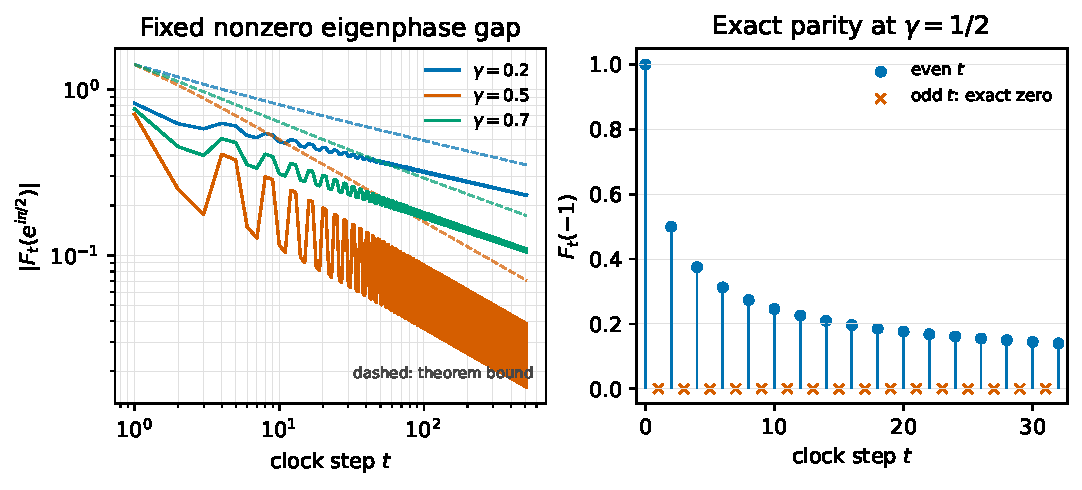
\includegraphics[width=0.91\textwidth]{figures/coherence-decay.pdf}
 \caption{Critical coherence coefficients.  (a) Absolute coefficients at the
 fixed eigenphase ratio $z=e^{i\pi/2}$ for three values of $\gamma$; dashed
 curves are the exact endpoint-mass bounds in
 Eq.~\eqref{eq:scalar-bound}.  (b) At $\gamma=1/2$ and $z=-1$, odd-time
 coefficients are exactly zero, while even-time coefficients equal
 $\binom{2q}{q}/4^q$.  Values were generated by
 Eq.~\eqref{eq:coefficient-recurrence}; the accompanying comma-separated
 table records every plotted value.  The plotting code and figure preparation
 used the AI assistance disclosed below; the coefficients were checked against
 an independent 80-digit convolution, the proved envelope, and the exact
 parity identity.}
 \label{fig:decay}
\end{figure*}

\section{Two boundary singularities and parity}
\label{sec:asymptotics}

For fixed $|z|=1$ with $z\ne1$, the generating function in
Eq.~\eqref{eq:F-generating} has two distinct algebraic singularities on its
circle of convergence, at $u=1$ and $u=z^{-1}$.  Expanding the analytic
cofactor at both points and applying the two-point Darboux coefficient
estimate~\cite{FlajoletSedgewick2009} gives
\begin{widetext}
\begin{equation}
 F_t(z)=(1-z)^{\gamma-1}a_t
 +(1-z^{-1})^{-\gamma}z^tb_t
 +O_{\gamma,z}\!\left(t^{\gamma-2}+t^{-\gamma-1}\right).
 \label{eq:darboux-ab}
\end{equation}
\end{widetext}
The branches are those inherited by the binomial series for $|u|<1$.
Subtracting the two displayed singular terms leaves local orders
$O((1-u)^{1-\gamma})$ at $u=1$ and $O((1-zu)^\gamma)$ at $u=z^{-1}$;
their coefficients give the two remainder powers in
Eq.~\eqref{eq:darboux-ab}.  The constants can be chosen uniformly for
$\gamma$ in a compact subset of $(0,1)$ and $|1-z|\geq\delta_0>0$, but not
as the two singularities merge.

Using the gamma-ratio expansions of $a_t$ and $b_t$ gives the leading form
\begin{widetext}
\begin{equation}
 F_t(z)=\frac{(1-z)^{\gamma-1}}{\Gamma(\gamma)}t^{\gamma-1}
 +\frac{(1-z^{-1})^{-\gamma}}{\Gamma(1-\gamma)}z^tt^{-\gamma}
 +O_{\gamma,z}\!\left(t^{\gamma-2}+t^{-\gamma-1}\right).
 \label{eq:darboux-power}
\end{equation}
\end{widetext}
The $u=z^{-1}$ contribution decays more slowly when $\gamma<1/2$, the
$u=1$ contribution decays more slowly when $\gamma>1/2$, and both are of
the same order at $\gamma=1/2$.  Keeping only the $u=1$ singularity would
miss the phase-dependent term relevant to unitary coherences.

The symmetric phase-$\pi$ point has an exact cancellation.  At
$\gamma=1/2$ and $z=-1$,
\begin{equation}
 \sum_{t\geq0}F_t(-1)u^t
 =(1-u)^{-1/2}(1+u)^{-1/2}=(1-u^2)^{-1/2},
 \label{eq:parity-gf}
\end{equation}
so
\begin{equation}
 \boxed{F_{2q+1}(-1)=0,\qquad
 F_{2q}(-1)=\frac{\binom{2q}{q}}{4^q}
 \sim\frac{1}{\sqrt{\pi q}}.}
 \label{eq:parity}
\end{equation}
This is a cancellation within convergence, not a resonance or a failure to
relax.

Figure~\ref{fig:decay} evaluates exact coefficients from
Eq.~\eqref{eq:F-generating}.  Differentiating that generating function gives
the recurrence
\begin{equation}
 \begin{split}
 (t+1)F_{t+1}(z)={}&\bigl[(1+z)t+\gamma+(1-\gamma)z\bigr]F_t(z)\\
 &{}-ztF_{t-1}(z),
 \end{split}
 \label{eq:coefficient-recurrence}
\end{equation}
with $F_0=1$ and $F_1=\gamma+(1-\gamma)z$.  The dashed curves use the
nonasymptotic right-hand side of Eq.~\eqref{eq:scalar-bound}; they are not
fits.  The second panel displays Eq.~\eqref{eq:parity} directly.

\section{Physical interpretation and limitations}

The limit $\cD_U(\rho_R)$ preserves precisely the coherences lying within a
degenerate eigenspace of the gate.  Every occupied coherence between distinct
gate eigenvalues is suppressed, even though the critical renewal time has
infinite mean.  The two endpoint masses have a direct renewal interpretation:
$a_t=P_0(t)$ weights a reset at the observation time, whereas
$b_t=P_t(t)$ weights an excursion with no reset after initialization.  Their
competing algebraic decays determine the slowest fixed-gap coherence scale.

The theorem is finite-dimensional in an essential way: only finitely many
occupied nonzero chord gaps enter Eq.~\eqref{eq:weighted-trace-bound}.  It does
not provide a bound uniform in a sequence of gates whose occupied gap closes,
nor does it exchange the long-time limit with a thermodynamic or
infinite-dimensional limit.  The endpoint values $\gamma=0,1$, hazards with
$\alpha\ne1$, mixed or partial reset rules, time-dependent gates, and
dissipative evolution between resets require separate analyses.  The norm in
Eqs.~\eqref{eq:weighted-trace-bound}--\eqref{eq:main-limit} is the Schatten
trace norm; the conventional trace distance is one half of it.

The numerical calculations accompanying this paper are diagnostics of the
closed forms and finite-register block identity.  They are not the certificate
for the infinite-time result: that certificate is the exact age law,
variation estimate, summation-by-parts identity, and finite spectral
decomposition above.

\section{Conclusion}

Critical Sibuya resetting prepares the $U$-pinched reset state on every fixed
finite unitary register.  A U-shaped exact age distribution supplies an
ordinary-time Fourier bound whose endpoint masses decay for all
$0<\gamma<1$, and the finite spectral decomposition turns it into an explicit
trace-norm estimate.  The two distinct unit-circle singularities explain the
phase-dependent algebraic rates and the exact half-Sibuya parity effect.  A
uniform closing-gap crossover and the full classification away from the
critical hazard remain open extensions.

\section*{Data availability}

No experimental or externally collected data were used.  The manuscript
source package includes the code and comma-separated data that regenerate
Fig.~\ref{fig:decay}, together with independent coefficient and finite-register
diagnostic programs.  The analytic result is self-contained in the displayed
identities and inequalities.

\section*{AI-assisted methods and disclosure}

OpenAI Codex, using the GPT-6 Astra and GPT-5.6 Sol model families, was used
substantively for literature synthesis, derivations, code generation,
diagnostic calculations, an independent model-context replay, figure
generation, and manuscript drafting.  The workflow fixed the model and claim
before review and checked outputs against versioned primary sources, exact
algebraic identities, independently implemented recurrences, and a separate
replay.  Artificial intelligence is not an author.  Before any submission,
the named author must independently review and refine all AI-assisted content,
confirm the tool terms and rights, and assume responsibility for the work.

\bibliography{references}

\end{document}
